\documentclass[10pt]{article}

\usepackage{mathtools}  % need for math tools
\usepackage{amsmath}    % need for subequations
\usepackage{graphicx}   % need for figures
\usepackage{verbatim}   % useful for program listings
\usepackage{color}      % use if color is used in text
\usepackage{subfigure}  % use for side-by-side figures
\usepackage{hyperref}   % use for hypertext links, including those to external documents and URLs
\usepackage{graphicx}   % Used to import the graphics
\usepackage{subfig}     % Used to creat subfigs

\setlength{\baselineskip}{16.0pt}   
\setlength{\parskip}{3pt plus 2pt}
\setlength{\parindent}{20pt}
\setlength{\oddsidemargin}{0.5cm}
\setlength{\evensidemargin}{0.5cm}
\setlength{\marginparsep}{0.75cm}
\setlength{\marginparwidth}{2.5cm}
\setlength{\marginparpush}{1.0cm}
\setlength{\textwidth}{150mm}



\begin{document}

\begin{center}
{\large Ay190: Computational Astrophysics (Winter Term 2012)} \\
{\large HomeWork - 4 (ODE and Root finding) } \\
\copyright 2012 by Arya Farahi \\
Jan 22, 2012
\end{center}

\section{Exercise 1. ODE Integration: Simplified Stellar Structure}

\begin{figure}[hbt]
  \centering
 \subfloat[Mass & Density]{ \label{fig:1} 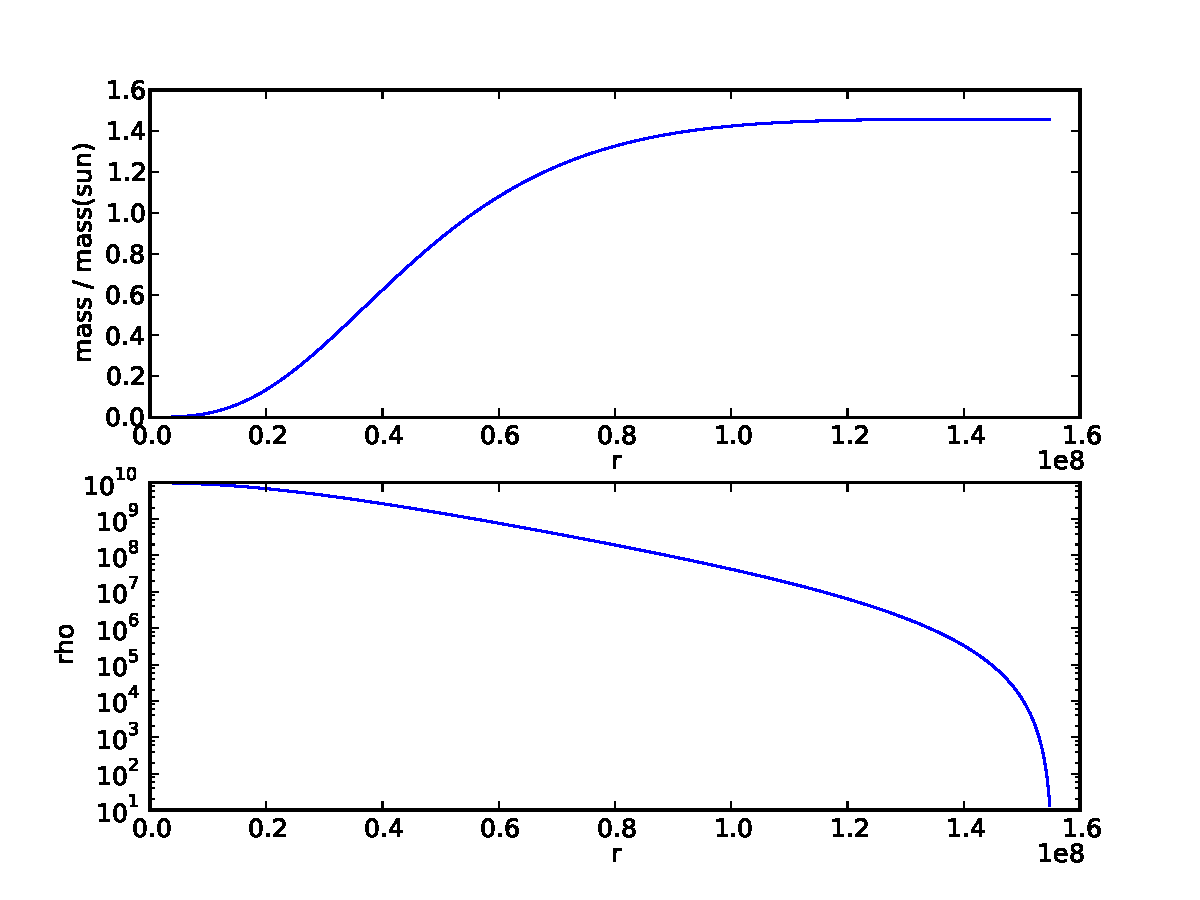
\includegraphics[scale=0.4]{Plot/plot1.pdf}}
 \subfloat[Pressure]{ \label{fig:2} 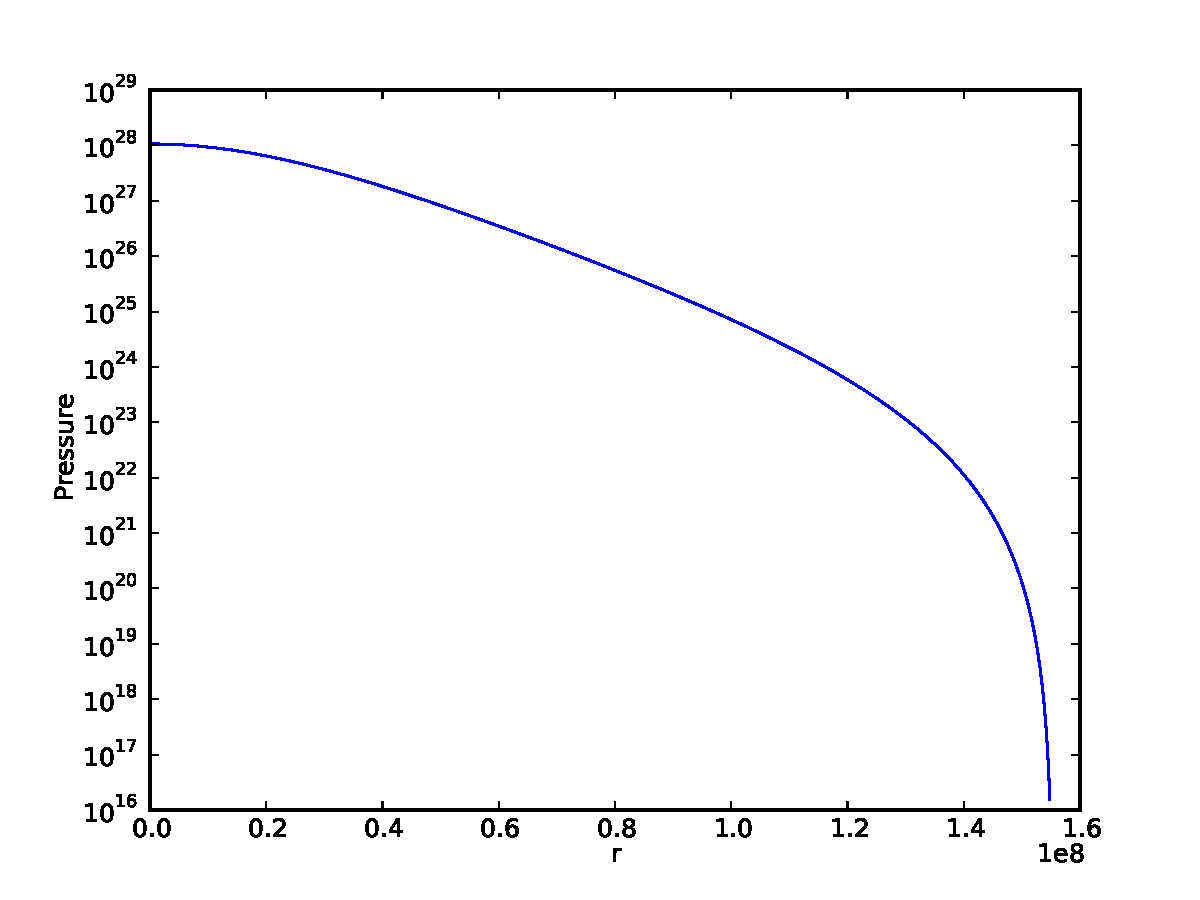
\includegraphics[scale=0.4]{Plot/plot2.pdf}}
    \caption{ Plot of the mass, density, and pressure of the star with changing radius.}
\end{figure}


\begin{figure}[hbt]
  \centering
    \subfloat[Self Convergence factor]{\label{fig:3} 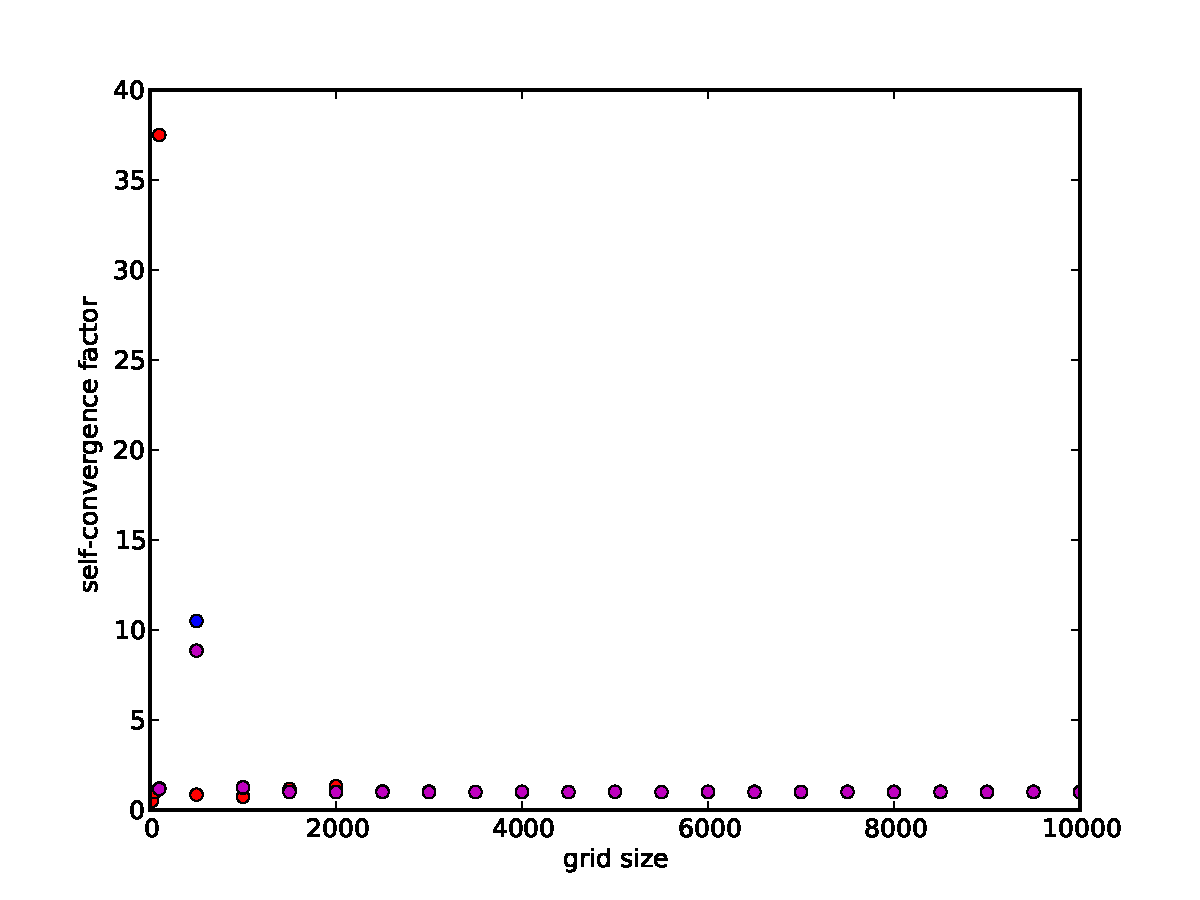
\includegraphics[scale=0.3]{Plot/plot3.pdf}}
    \subfloat[Relative error]{\label{fig:4} 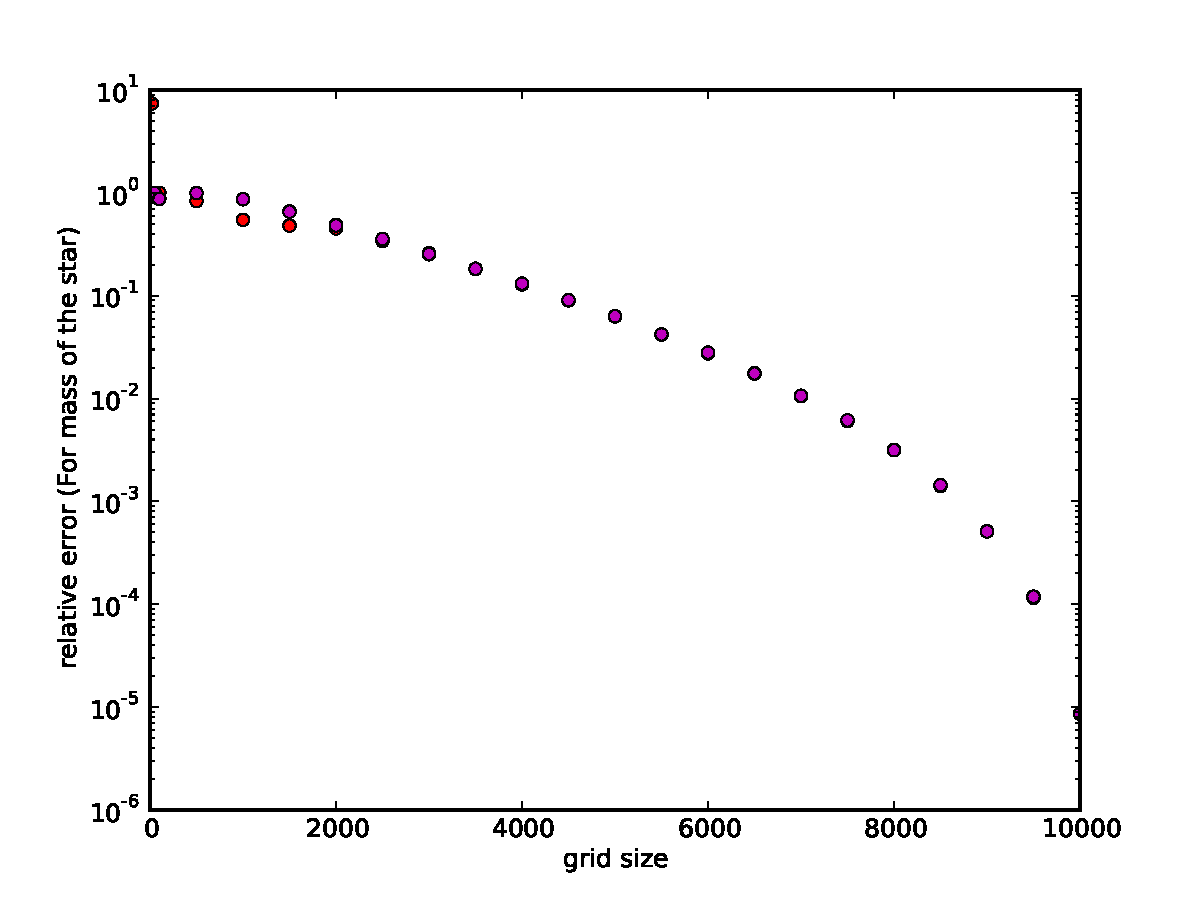
\includegraphics[scale=0.3]{Plot/plot4.pdf}}
    \caption{ Self Convergence factor with changing grid size and Relative error of the mass of star with changing grid size.}
\end{figure}


Figure \ref{fig:1} and \ref{fig:2} showes the plot of the mass of the star, its density, and its pressure with changing radius. Also the after the convergence it can be shown that mass of the star would be equal to $1.4574 \times M_{\odot}$and its radius would be equal to $154850 km$.
Figure \ref{fig:3} and \ref{fig:4} shows that our solution is converging. Figure \ref{fig:3} is the Self Convergence factor which is changing with grid size and Figure \ref{fig:4} is the Relative error of the mass of star which is changing with grid size. It is obvious that for all three methods the numerical solution converge to real answer. \\

\pagebreak

\section{Exercise 2. Root Finding: Eccentricity Anomality}

\bfseries{Part a : } \\ \mdseries
In this problem I used Newton’s Method for finding the root of equation $f(E) = E - \omega t - e \sin E$. So we need to find its derivitive respect to $E$. We find its derivitive analyticaly which is $F'(E) = 1 - e \cos E$. And for the initial trial I used  $E = 0$ and with just 4 trial the answer converge. Then for $t = 91$ days, $t = 182$ days,and $t = 273$ days $E$ would be equal to $1.58$, $3.13$, and $4.67$ respectively.

\bfseries{Part b :}\\ \mdseries

I used the same method for the second part of the problem. But if we want to use $E = 0$ as our initial rtial then the method would not converge to the root of the function. But if we change the initial trial with small number of trial we are able to find the answer, just with 7 tial. And for $t = 91$ days, $t = 182$ days,and $t = 273$ days $E$ would be equal to $2.30$, $3.13$, and $3.967$ respectively.\\

 The density of electrons in this environment by useing Gauss-Laguerre Quadrature and Trapezoidal Rule method for finding the numerical integral is same and it is equal to : $1.90216 \times 10^{41}$. We used 50 pionts for finding the answer of integral.\\

Figure \ref{fig:5} and \ref{fig:6} shows the the relative error with changing the number of trial for part a and part b of the problem. 

\begin{figure}[hbt]
  \centering
    \subfloat[91 days]{ 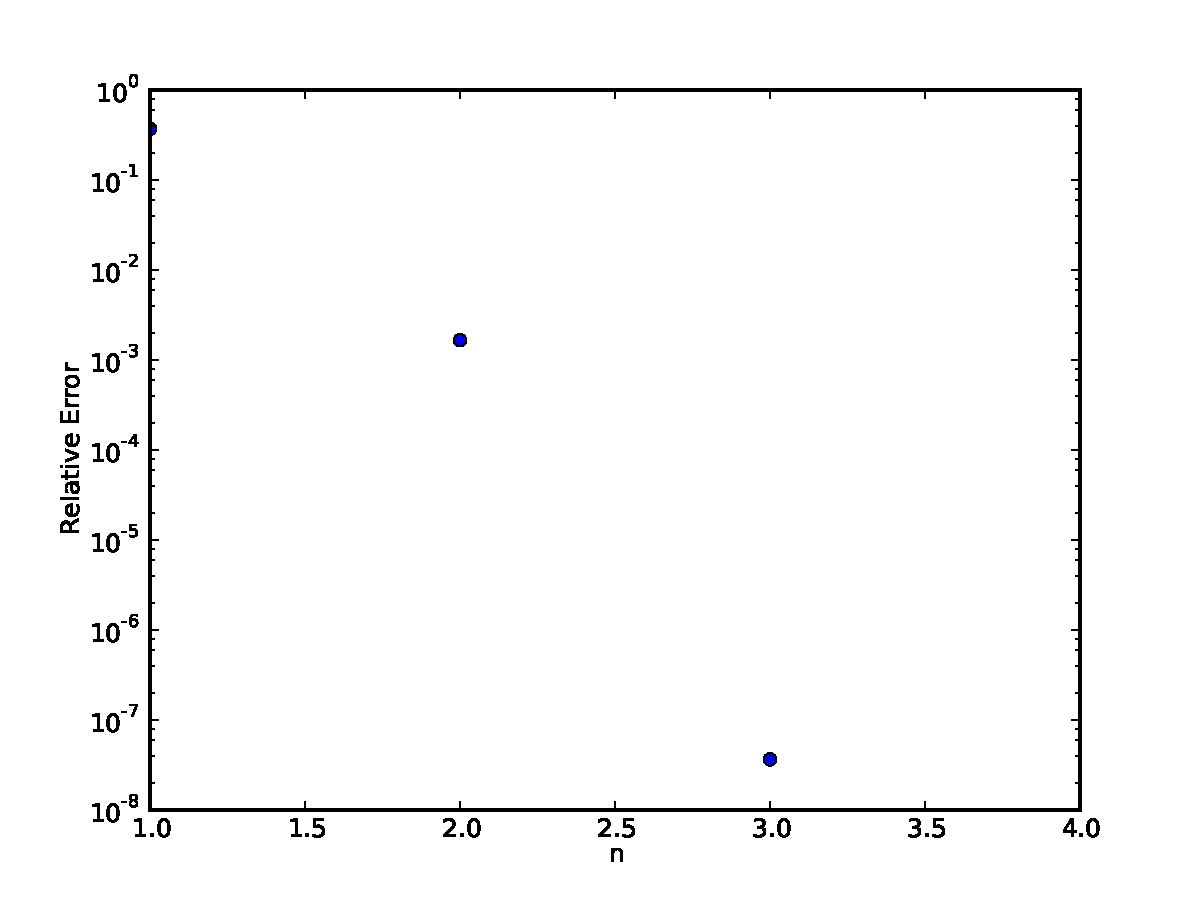
\includegraphics[scale=0.2]{Plot/plotI0.pdf}}
    \subfloat[182 days]{ 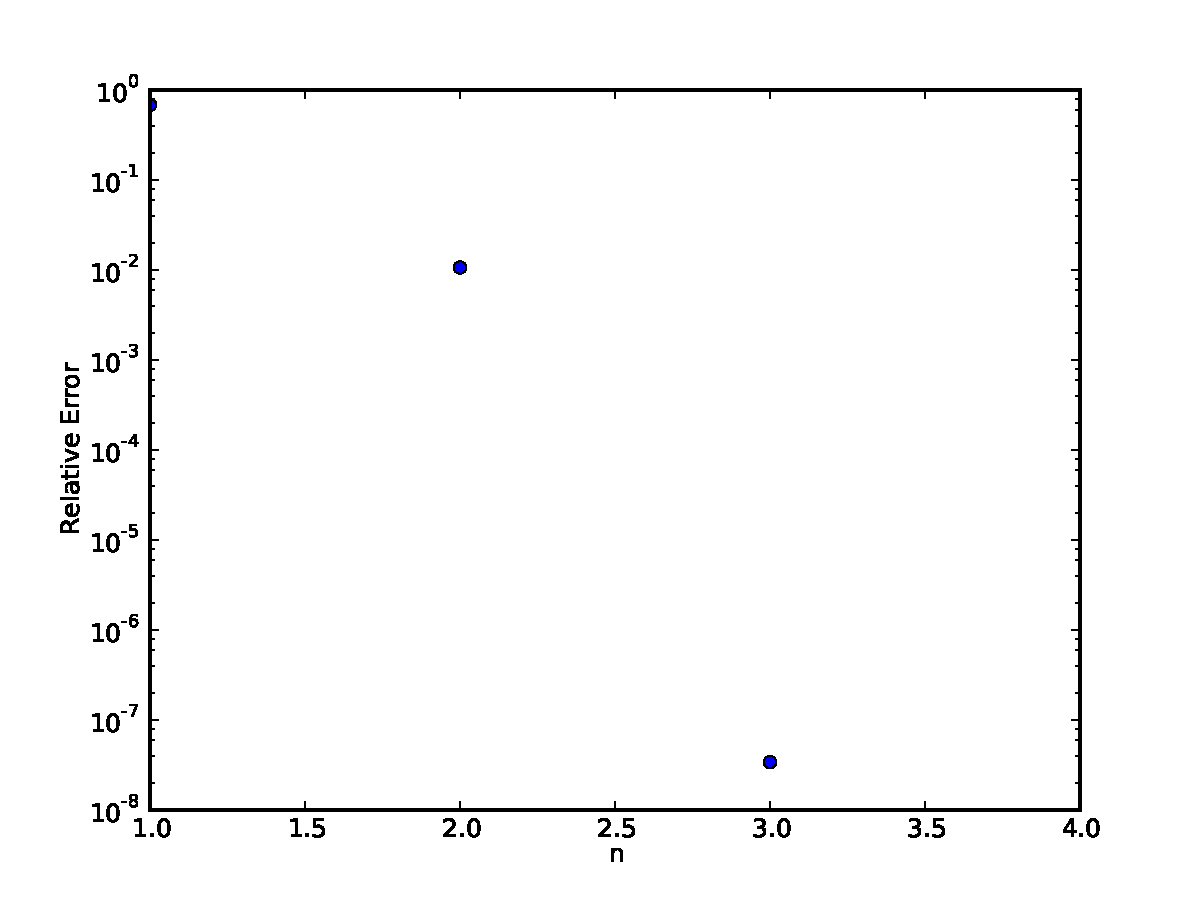
\includegraphics[scale=0.2]{Plot/plotI1.pdf}}
    \subfloat[273 days]{ 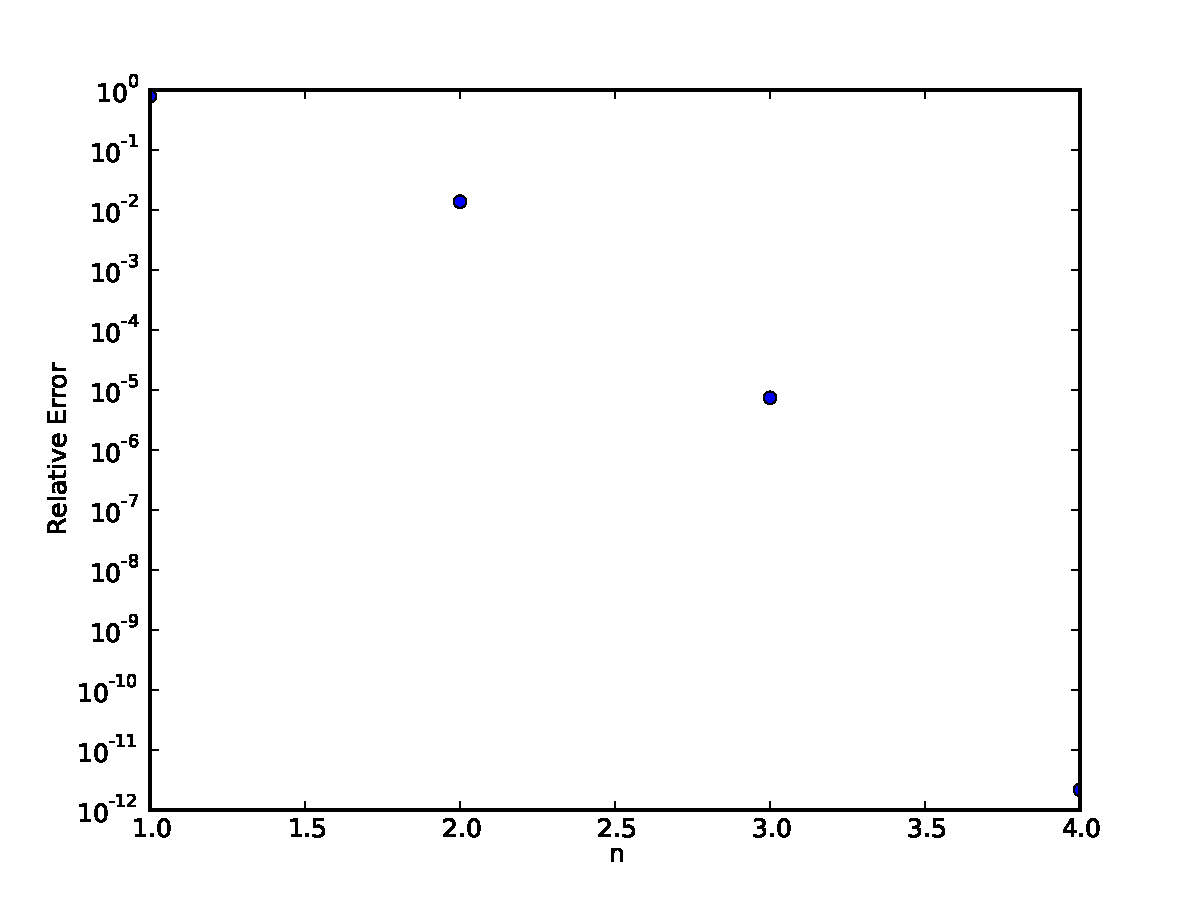
\includegraphics[scale=0.2]{Plot/plotI2.pdf}}
    \caption{ \label{fig:5} Plot of Relative error of $E$ with changing the number of tiral for $e = 0.0167$.}
\end{figure}


\begin{figure}[hbt]
  \centering
    \subfloat[91 days]{ 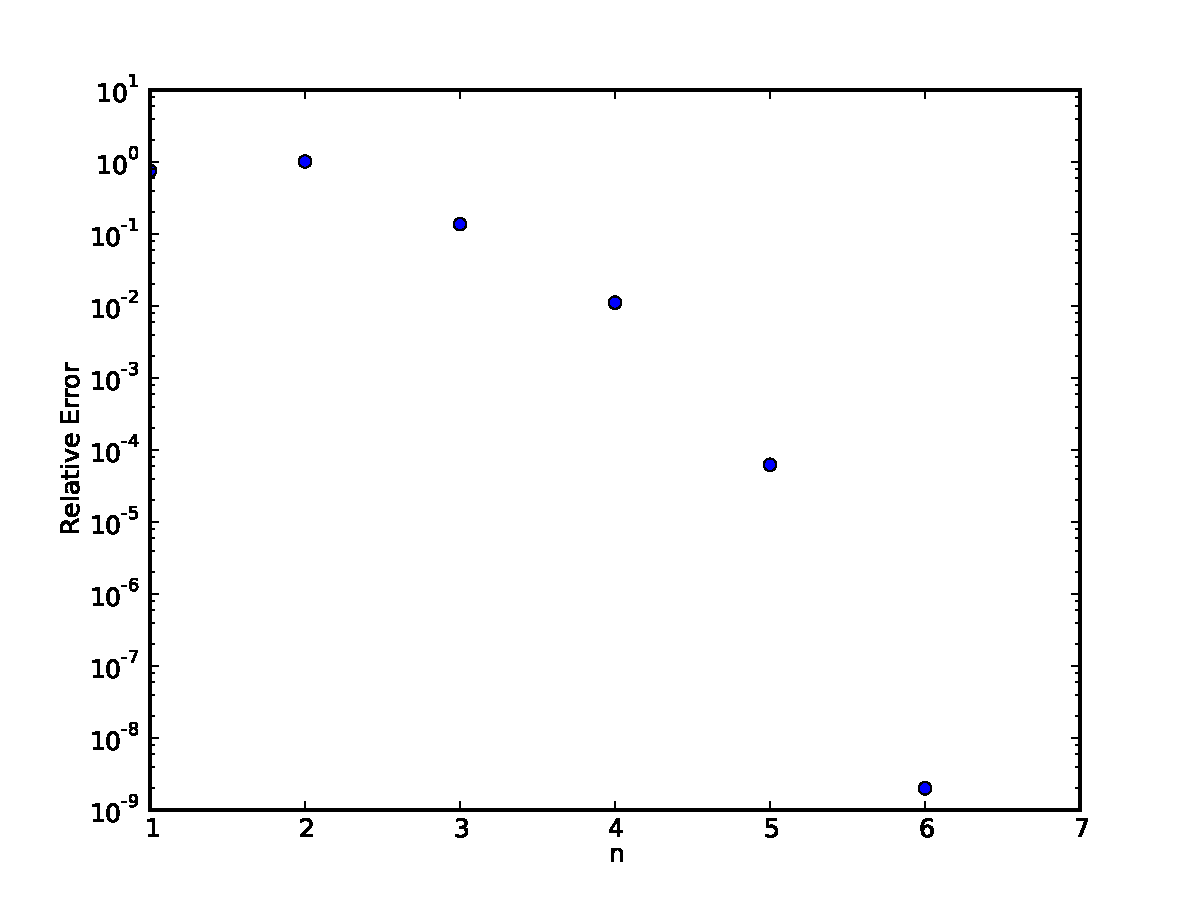
\includegraphics[scale=0.2]{Plot/plotII0.pdf}}
    \subfloat[182 days]{ 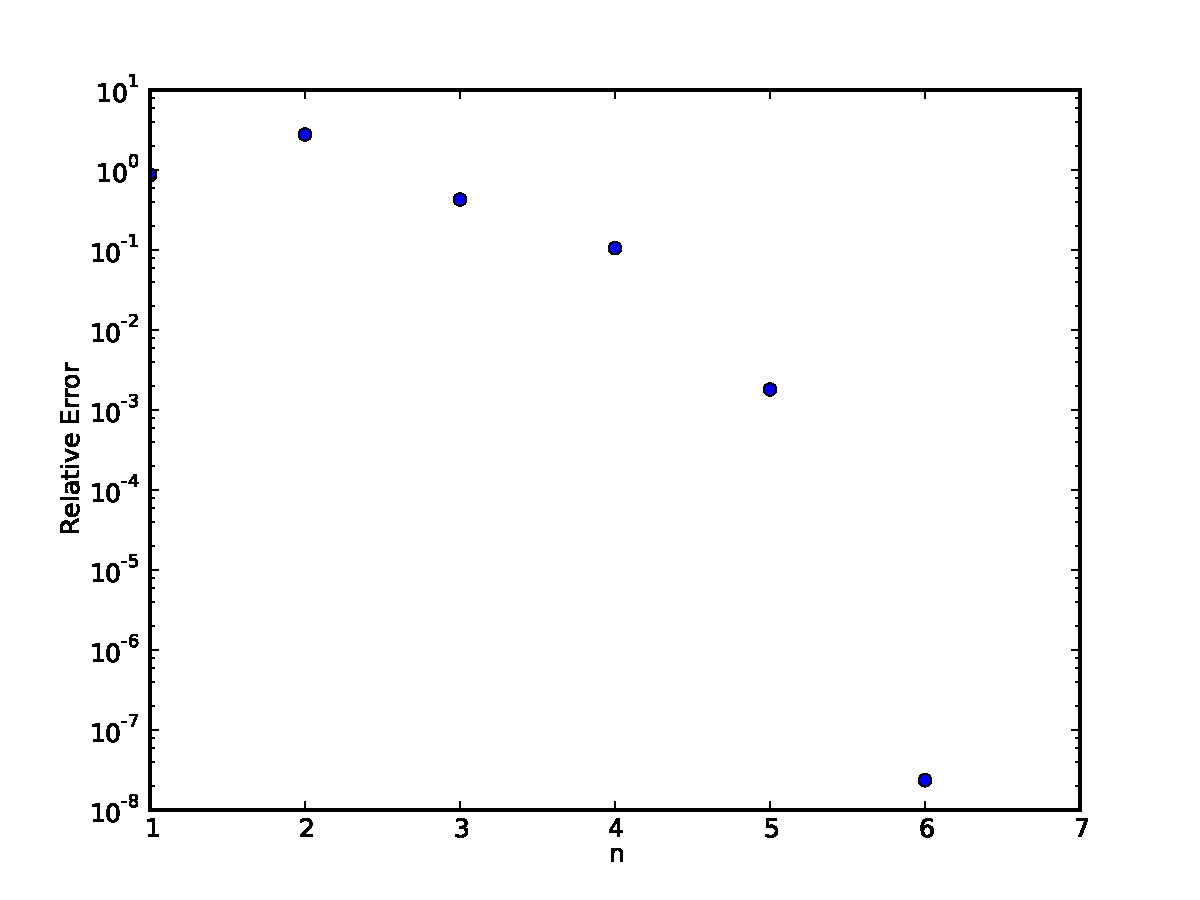
\includegraphics[scale=0.2]{Plot/plotII1.pdf}}
    \subfloat[273 days]{ 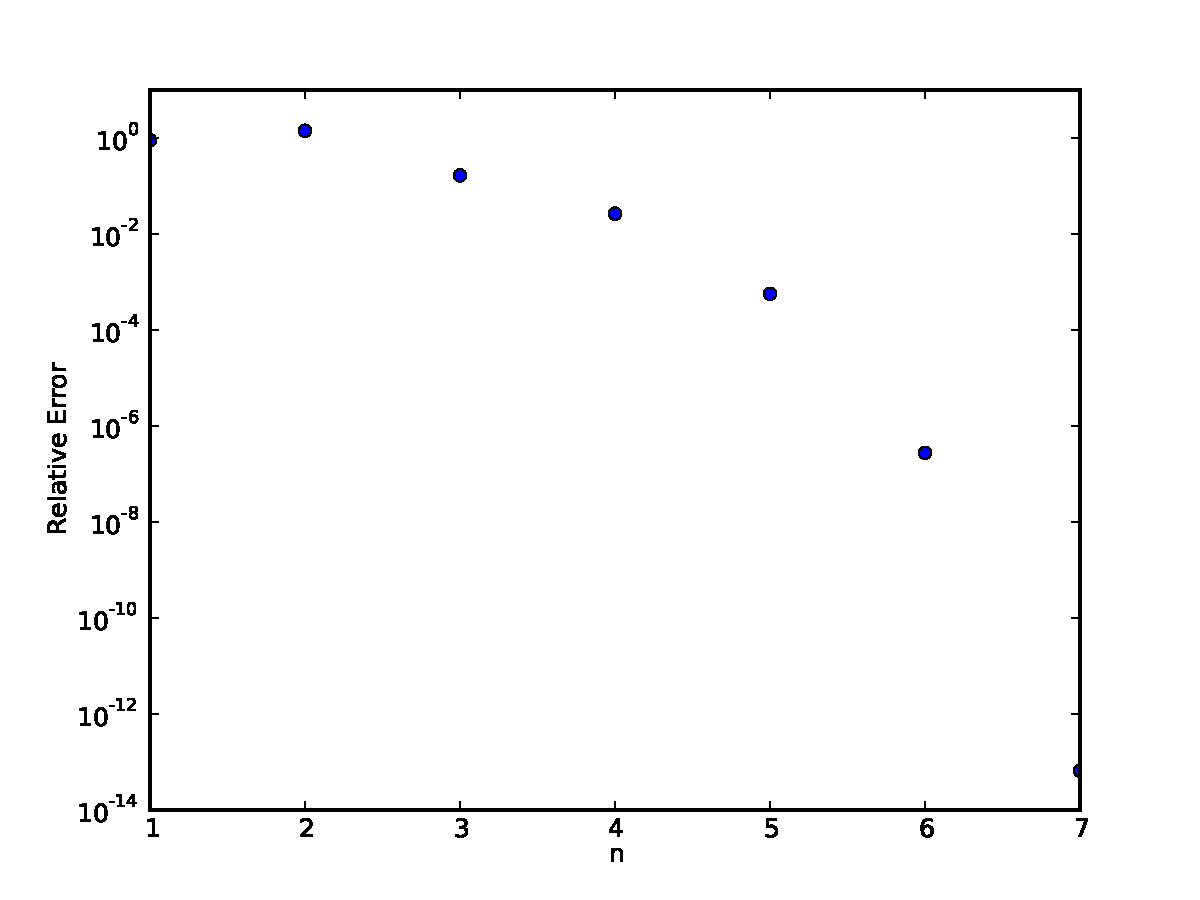
\includegraphics[scale=0.2]{Plot/plotII2.pdf}}
    \caption{ \label{fig:6} Plot of Relative error of $E$ with changing the number of tiral for $e = 0.99999$.}
\end{figure}

\section{Exercise 3. }

In this problem we want to find the roots of the polynomial functions. As we know for continous functions (such as polynomial function) the roots are exist between two extremum or after the last extremum or befor the first extremum or just located on the extremum. And in each situation there is only one root so we can find the roots by just knowing the extremums of the function and using the Newton method for example.\\

For finding the extremum we neet to find the roots of first derivative of function. And for finding the roots of the first derivative of function we neet to find the extremum of that and for that perpose we neet to find the roots of second derivative of function of our function and so on. Fortunatly there is limited of steps for polynomial function. Because the $n^{th}$ derivative of polynomial function is constant and after that the others derivatives are all zero. So we need to do this step just n-1 times and then we are able to find the roots of our function.\\

I have used several functions to calculate the $n^{th}$ derivative and finding the roots (extremums) and the check if there is any root between extrimums or not. And by this way I have found all the roots of our main function.\\ 


\end{document}
